\documentclass[a4paper,oneside,12pt, extrafontsizes]{memoir}

\usepackage{graphicx}
\usepackage{verbatim}
\usepackage{amsthm}

\theoremstyle{definition}
\newtheorem*{definition}{Definition}

\theoremstyle{definition}
\newtheorem*{examples}{Examples}

\theoremstyle{definition}
\newtheorem*{concrete-syntax}{Concrete Syntax}

\theoremstyle{definition}
\newtheorem*{abstract-syntax}{Abstract Syntax}

\theoremstyle{definition}
\newtheorem*{constraints}{Constraints}

\renewcommand{\familydefault}{\sfdefault}
\chapterstyle{demo2}

\usepackage{hyperref}
\hypersetup{pdftex,colorlinks=true,allcolors=blue}
\usepackage{hypcap}

\usepackage{color}
\definecolor{dark_blue}{rgb}{0.0,0.0,0.7}
\definecolor{fielddrab}{rgb}{0.42, 0.33, 0.12}

\usepackage{textcomp}
\usepackage{listings}
\lstset{upquote=true,basicstyle=\footnotesize,frame=single}
\lstdefinelanguage{cml}
{
  identifierstyle=\color{dark_blue},
  morestring=[b]",
  stringstyle=\color{fielddrab},
  morecomment=[l]{--},
  commentstyle = \color{black},
  morekeywords={,abstract,concept,task,association,select,reject,
  yield,recurse,count,first,last,if,then,else,for,in,}
}
\lstdefinelanguage{antlr}
{
  identifierstyle=\color{dark_blue},
  morestring=[b]",
  stringstyle=\color{fielddrab},
  morekeywords={,returns,}
}
\lstdefinelanguage{lsl}
{
  identifierstyle=\color{dark_blue},
  morestring=[b]',
  stringstyle=\color{fielddrab},
  morecomment=[l]{//},
  commentstyle = \color{black},
  morekeywords={,node,select,reject,
  yield,recurse,count,first,last,if,then,else,for,in,}
}
\lstdefinelanguage{ocl_}
{
  identifierstyle=\color{dark_blue},
  morestring=[b]',
  stringstyle=\color{fielddrab},
  morecomment=[l]{--},
  commentstyle = \color{black},
  morekeywords={,self,context,inv,pre,post,and,or,implies,derive,body,if,then,else,}
}

\title{\emph{Conceptual Modeling Language}\\Specification\\ \small{Version 1.0 (Draft)}}
\author{Quenio Cesar Machado dos Santos\\
\small{Universidade Federal de Santa Catarina}\thanks{
Initially developed as part of the author's Bachelor Technical Report in Computer Sciences}}
\date{July 2017}

\makeatletter
\newcommand{\verbatimfont}[1]{\renewcommand{\verbatim@font}{\ttfamily#1}}
\makeatother

\makeatletter
\renewcommand*{\p@chapter}{\S\,}
\renewcommand*{\p@section}{\S\,}
\renewcommand*{\p@subsection}{\S\,}
\makeatother

\begin{document}

\begin{titlingpage}
\maketitle
\end{titlingpage}

\frontmatter

\begin{KeepFromToc}

\clearpage
\tableofcontents

\clearpage
\listoffigures

\clearpage
\listoftables

\end{KeepFromToc}

\mainmatter

\chapter{Introduction}
This document specifies the \emph{Conceptual Modeling Language}, or CML for short.
CML enables the modeling of the information of software systems.
It focuses on modeling the structural aspects of such systems,
having less emphasis on the behavioral aspects.
Using CML,
it is possible to represent the information as understood by the system users,
while disregarding its physical organization as implemented by target languages or technologies.

The CML compiler has:
\begin{itemize}
\item as \emph{input},
source files defined using its own conceptual language (as specified in this document),
which provides an abstract syntax similar to (but less comprehensive than) a combination of UML \cite{uml} and OCL \cite{ocl};
\item and, as \emph{output},
any target languages based on extensible templates,
which may be provided by the compiler's base libraries, by third-party libraries, or even by developers.
\end{itemize}

Section \ref{sec:compiler} will provide an overview of the CML compiler's architecture.
Section \ref{sec:org} describes the organization and notation
used in the remainder of this document.


\section{The CML Compiler}
\label{sec:compiler}
The CML compiler's overall architecture follows the standard compiler design literature \cite{torben}. An overview diagram of the architecture is shown in figure \ref{fig:overview}.

\begin{figure}
\centering
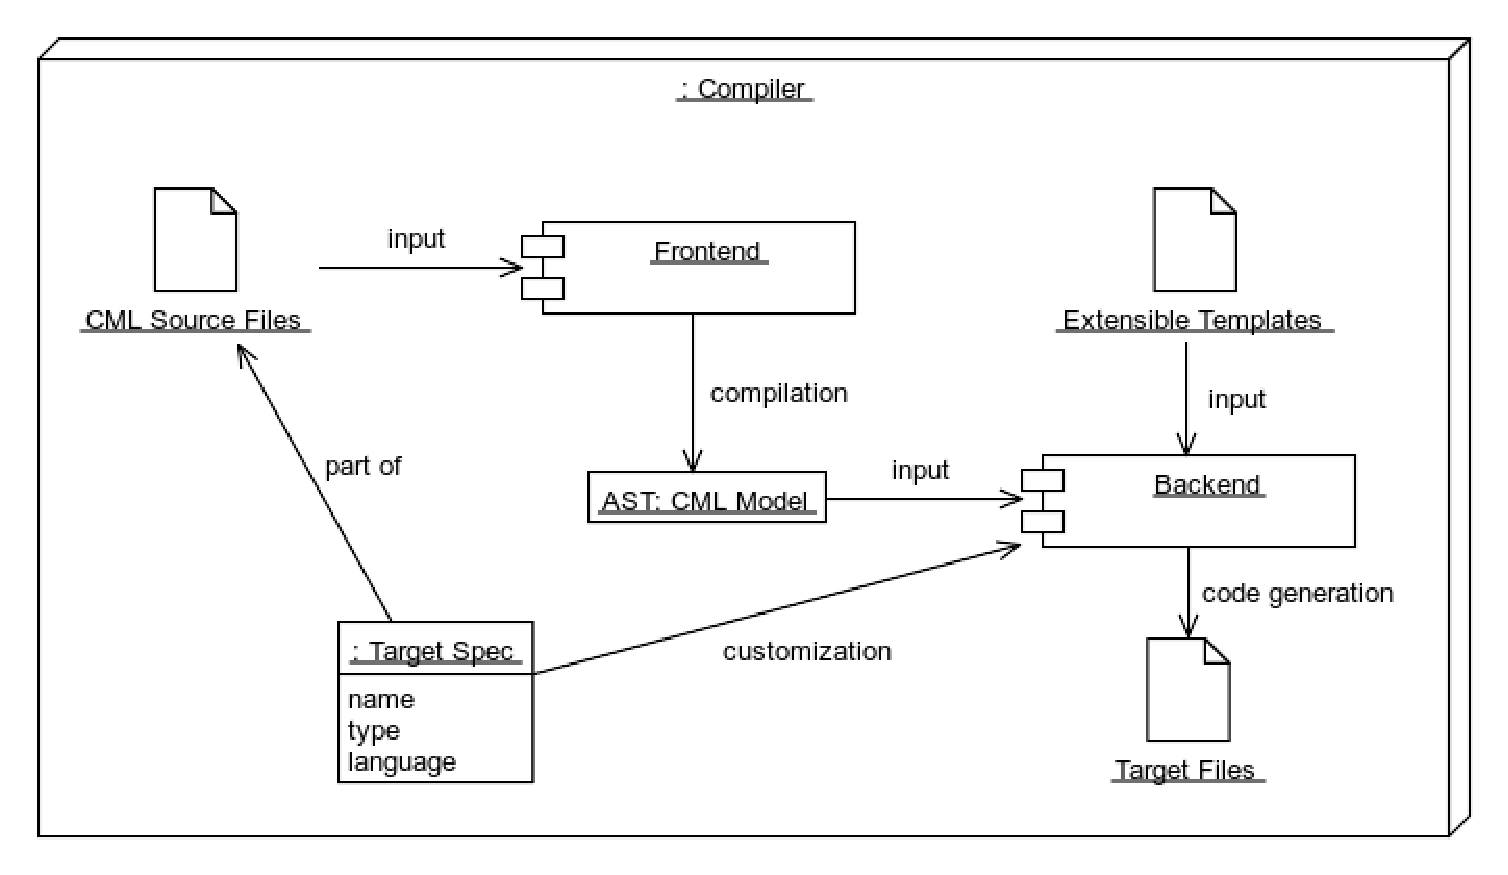
\includegraphics[width=\textwidth]{compiler/figure-overview}
\caption{An architectural overview of the CML compiler.}
\label{fig:overview}
\end{figure}

The two main components of the compiler,
and the artifacts they work with,
are presented in the next subsections.


\subsection[Frontend]{The Compiler Frontend}
\label{subsec:frontend}
The frontend receives as input the \emph{CML source files}.
It will parse the files and generate an internal representation of the \emph{CML model}.

Syntactical and semantic validations will be performed at this point.
Any syntax and constraint errors are presented to the developer, interrupting the progress to the next phase.
If the \emph{source files} are parsed and validated successfully, then the internal representation (the AST) of the \emph{CML model} is provided as the input for the \emph{backend} component.


\subsection[Backend]{The Compiler Backend}
\label{subsec:backend}
The backend receives the \emph{CML model AST} as input.
Based on the \emph{target specification} provided by the AST, chooses which \emph{extensible templates} to use for code generation.
The \emph{target files} are then generated, and become available to be consumed by other tools. The \emph{task declaration} plays the key role of determining the kind of \emph{target} to be generated.

CML extensible templates are implemented in StringTemplate \cite{st}.  The CML compiler uses StringTemplate for two purposes:

\begin{itemize}
\item \emph{File names and directory structure:}
each type of target generated by the CML compiler requires a different directory structure.
The CML compiler expects each target type to define a template file named ``files.stg'' (also known as \emph{files template}),
which will contain the path of all files to be generated. The \emph{files template} may use information provided by the \emph{task declaration}
in order to determine the file/directory names.
\item \emph{File content generation:}
each file listed under the \emph{files template} will have a corresponding \emph{content template} that specifies how the file's content must be generated. The \emph{content template} will receive as input one root-level element of the CML model, which will provide information to generate the file's content.
Each type of top-level model element should have a corresponding \emph{content template}. Templates are described in \emph{Code Generation} part of this specification.
\end{itemize}


\section{Organization and Notations}
\label{sec:org}
The following chapters will specify every element of CML metamodel.
Each chapter starts with a definition, followed by: an example;
the specification of the concrete syntax;
and then presenting the abstract syntax,
and how to transform the concrete syntax into the abstract one.

Chapters may also have sections that specify sub-elements
of the top-level CML metamodel element being described in the chapter level.
Each sub-element is described under its section
using the same definition structure (detailed below)
that is used to define the top-level elements.

\begin{definition}
The definition of each CML metamodel element is stated in plain English
on a paraprah (such as this one)
starting with the ``\textbf{Definition.}'' heading.
If a correspondence exists to an element of
the Entity-Relationship (ER) \cite{er} metamodel,
or to an element of the Unified Modeling Language (UML) \cite{uml} metamodel,
it is provided.
\end{definition}

\begin{examples}
For each metamodel element declaration in CML,
examples are provided on a paraprah (such as this one),
starting with the ``\textbf{Examples.}'' heading.
This type of paragraph refers to a \verb+verbatim+ figure
containing the examples, and describes them as needed.
The examples are provided for illustrative purposes only,
and they are \emph{not} intended to be normative.
They may be excerpts of larger CML source files,
and thus may not be successfully compiled on their own.
\end{examples}

\begin{concrete-syntax}
The concrete syntax of each CML metamodel element is described
on a paragraph (such as this one),
starting with the ``\textbf{Concrete Syntax.}'' heading.
This type of paragraph refers to a \verb+verbatim+ figure,
which contains the actual ANTLR \cite{antlr} grammar
specifying the syntax for the CML metamodel element in question,
and it must be considered normative.
The appendix \ref{apx:concrete-syntax} presents all the grammar rules
in a single listing.
\end{concrete-syntax}

\begin{abstract-syntax}
The abstract syntax of each CML metamodel element is described
on a paragraph (such as this one),
starting with the ``\textbf{Abstract Syntax.}'' heading.
This type of paragraph refers to two types of figure:
the first figure presents a class diagram
with the EMOF \cite{mof}-based metamodel
of the element being described;
the second figure specifies the transformation
from the concrete syntax into instances of the metamodel classes,
which are the nodes of the abstract syntax tree
(the intermediate representation described in section \ref{sec:compiler}).
The notation used to specify the transformations is presented
in the appendix \ref{apx:lsl}.
Both figures must be considered normative.
\end{abstract-syntax}

\begin{constraints}
The constraints of each CML metamodel element are described
on a paragraph (such as this one),
starting with the ``\textbf{Constraints.}'' heading.
This type of paragraph refers to a \verb+verbatim+ figure,
which contains the OCL \cite{ocl} invariants
(and its definitions)
of the CML metamodel element in question,
and it must be considered normative.
Each invariant has a name in the format \verb+inv_name+
so that it can be referred by the compiler's error messages
and users.
Derived properties may also be defined before the constraints
in order to simplify the constraint expressions.
The appendix \ref{apx:ocl} presents all the constraint rules
in a single listing.
\end{constraints}

All metamodel elements referred by one of the descriptions defined above
(definitions, examples, etc.)
are emphasized in \emph{italic}.
If the descriptions of a CML metamodel element refer to another CML metamodel element,
the corresponding chapter or section defining the other element
is provided in parenthesis, like so (\ref{sec:org}).

Some sections may not follow the structure defined above.
These normally provide additional semantic information in plain English,
which cannot be described using the notations presented above.


\chapter{Concepts}
\label{ch:concepts}

\begin{figure}
\verbatimfont{\small}
\begin{framed}
\verbatiminput{grammar/Concepts.txt}
\end{framed}
\caption{Concept Declaration Syntax}
\label{fig:concept-syntax}
\end{figure}

\section{Properties}\label{sec:properties}

\begin{figure}
\verbatimfont{\small}
\begin{framed}
\verbatiminput{grammar/Properties.txt}
\end{framed}
\caption{Properties Declaration Syntax}
\label{fig:properties-syntax}
\end{figure}

\section{Inheritance}\label{sec:inheritance}


\section{Properties}
\label{sec:properties}
\begin{definition}
A \emph{property} in CML may hold values of primitive types,
in which case they correspond to \emph{attributes}
on the ER \cite{er} and UML \cite{uml} metamodels;
or they may hold references (or collections of references)
linking to instances of other \emph{concepts},
in which case they correspond to a \emph{relationship} on the ER metamodel,
and to \emph{associations} on the UML metamodel.
\end{definition}

\begin{examples}
Figure \ref{fig:ex:properties} presents some examples of \emph{properties} declared in CML.
As shown in the examples,
a \emph{property} may be an \emph{attribute} (\ref{ch:attributes})
of a \emph{primitive type} (\ref{sec:primitive-types}),
or represent the role/end of an \emph{association} (\ref{ch:associations}).
\end{examples}

\begin{figure}
\verbatimfont{\small}
\begin{framed}
\verbatiminput{examples/properties.cml}
\end{framed}
\caption{Property Examples}
\label{fig:ex:properties}
\end{figure}

\begin{concrete-syntax}
Figure \ref{fig:stx:property} specifies the syntax used
to declare a \emph{property}.
The NAME is followed by a \emph{typeDeclaration}
(\ref{sec:primitive-types} and \ref{sec:collection-types}).
Optionally, an \emph{expression} (\ref{ch:expressions}) may be specified
in order to set the initial value.
\end{concrete-syntax}

\begin{figure}
\verbatimfont{\small}
\begin{framed}
\verbatiminput{grammar/Properties.txt}
\end{framed}
\caption{Property Declaration Syntax}
\label{fig:stx:property}
\end{figure}

\begin{abstract-syntax}
Figure \ref{fig:meta:property} presents the \emph{property} metamodel
in an EMOF \cite{mof} class diagram,
and figure \ref{fig:ast:property} specifies
the transformation
from the \emph{property} concrete syntax to its abstract syntax.
For each \emph{property} parsed by the compiler,
an instance of the \emph{Property} class will be created,
and its properties will be assigned
according to parsed information:

\begin{itemize}

\item \emph{name}:
assigned with the value of the terminal node NAME.

\item \emph{type}:
if \emph{typeDeclaration} is provided,
\emph{type} is set with the instance of the \emph{Type} class
matching the \emph{typeDeclaration}.

\item \emph{expression}:
if \emph{expression} is provided,
it contains the instance of the \emph{Expression} class
matching the parsed \emph{expression}.

\end{itemize}
\end{abstract-syntax}

\begin{figure}
\verbatimfont{\small}
\begin{framed}
\verbatiminput{ast/property.lsl}
\end{framed}
\caption{Property AST Instantiation}
\label{fig:ast:property}
\end{figure}


\section{Generalization / Specialization}
\label{sec:generalization}
\begin{definition}
A \emph{concept} in CML may specialize another one,
which is the same as saying that a \emph{concept} is generalized by another one.
In the UML \cite{uml} metamodel,
this generalization/specialization relationship between \emph{classes}
is known as \emph{generalization}, which is the name of the metaclass in the metamodel.
The original version of the ER \cite{er} metamodel lacked this kind of relationship.
\end{definition}

\begin{figure}
\verbatimfont{\small}
\lstinputlisting[language=cml]{examples/generalization.cml}
\caption{Generalization Examples}
\label{fig:ex:concepts}
\end{figure}


\section{Abstract Concepts}
\label{sec:abstract}
\begin{definition}
An \emph{abstract concept} is one that does not represent specific instances,
but instead serves as a \emph{generalization} (\ref{sec:generalization}) 
for other \emph{concepts},
which in turn represent specific instances.
Thus, all instances of an \emph{abstract concept}
are first instances of its \emph{specializations}.
CML supports tagging a \emph{concept} as \emph{abstract}.
An \emph{abstract concept} in CML may also define a \emph{derived property} (\ref{sec:properties})
wihtout providing an \emph{expression} (\ref{ch:expressions}) in its definition;
such \emph{properties} may also be called \emph{abstract properties}.
CML's support for \emph{abstract concepts} matches UML's \cite{uml},
which allows the declaration of \emph{abstract classes}
-- by setting the \emph{isAbstract} attribute of the \emph{Class} metaclass instance to \emph{true}.
UML also allows the declaration of corresponding \emph{abstract attributes} and \emph{abstract operations}.
The original version of the ER \cite{er} metamodel, however,
as a consequence of lacking the \emph{generalization/specialization} relationship,
has not considered the notion of \emph{abstract entities}.
\end{definition}

\chapter{Attributes}
\label{ch:attributes}
\begin{definition}
In CML, \emph{attributes} are \emph{properties} (\ref{sec:properties})
of \emph{primitive types} (\ref{sec:primitive-types}).
They correspond to the \emph{Attribute} metaclass 
in the ER \cite{er} and UML \cite{uml} metamodels.
\emph{Attributes} serve as a \emph{slot} to hold a value of 
the specified \emph{primitive type}.
An initial value may be specified as an \emph{expression} (\ref{ch:expressions}).
An \emph{attribute}'s value may also be constantly
derived from an \emph{expression} (not only initially),
in which case it is called a \emph{derived attribute} (\ref{sec:derived-attributes}).
While initial values are only set when a \emph{concept} (\ref{ch:concepts})
is instantiated,
the value of \emph{derived attributes} are always evaluated 
from the given \emph{expression},
and they cannot be set any other way.
\end{definition}

\begin{examples}
Figure \ref{fig:ex:attributes} presents some examples of \emph{attributes} declared in CML.
As shown,
the attribute \textbf{a} is a regular attribute definition 
that specifies the \emph{primitive type} (\ref{sec:primitive-types})
of the values that can be held by the \emph{attribute}'s slot.
The attribute \textbf{b} is an example showing how an \emph{attribute}
can be defined with an initial value.
As shown by the attribute \textbf{c}, 
an attribute may be derived from an \emph{expression}
that refers to other \emph{attributes}.
In order to differentiate \emph{attributes} with initial values
from \emph{derived attributes},
a forward slash (``/'') prefixes the name of the latter.
Attributes \textbf{d} and \textbf{e} are examples
where the type of the attribute,
instead of being specified,
is inferred from the given \emph{expression}.
Type inference is possible for both slot-based \emph{attributes}
and \emph{derived attributes} that provide an \emph{expression}.
\end{examples}

\begin{figure}
\verbatimfont{\small}
\lstinputlisting[language=cml]{examples/attributes.cml}
\caption{Examples of Attributes}
\label{fig:ex:attributes}
\end{figure}


\section{Primitive Types}
\label{sec:primitive-types}
\begin{definition}
A \emph{primitive type} in CML is one of the pre-defined \emph{data types}
supported by the language,
as shown in tables \ref{tab:core-primitive-types} and \ref{tab:additional-primitive-types}.
In the ER \cite{er} metamodel,
a \emph{data type} is formally defined as a \emph{set} of \emph{values}
that can be held by an \emph{attribute} (\ref{ch:attributes}).
The original ER paper \cite{er} states that,
for each \emph{value set} (i.e. \emph{data type}),
there is a \emph{predicate} that can be used to test
whether a \emph{value} belongs to the \emph{set}.
In CML, instead,
\emph{literal expressions} are syntactically defined for each \emph{primitive type},
so that the \emph{type} can be inferred from the \emph{literal expression}.
On the original ER paper,
it is also said that \emph{values} in a \emph{value set}
may be equivalent to \emph{values} in another \emph{value set}.
In CML, also,
\emph{literal expressions} of the \emph{Integer} type may be equivalent 
to \emph{literal expressions} of the \emph{Decimal},
and so with other \emph{numeric types}.
This allows \emph{expressions} of a \emph{primitive type}
to be promoted to \emph{expressions} of another \emph{primitive type}
in order to allow \emph{type inference} of composite \emph{expressions},
such as \emph{infix expressions} (\ref{sec:infix}).
In the UML \cite{uml} metamodel,
there is a specific metaclass named \emph{PrimitiveType},
which matches to the same notion in CML.
\end{definition}

\begin{table}[h]
\centering
\begin{tabular}
{l l l l l p{2cm} }
\hline
CML & Java & C\# & C++ & Python & TypeScript (JavaScript) \\
\hline
String & String & string & std::wstring & str & string \\
\multicolumn{6}{p{13cm}}{\footnotesize{16-bit Unicode character sequences.}} \\
\\
Boolean & boolean & bool & bool & bool & boolean \\
\multicolumn{6}{p{13cm}}{\footnotesize{Only values are the literal expressions: \textbf{true}, \textbf{false}.}}  \\
\\
Integer & int & int & int32\_t & int & number  \\
\multicolumn{6}{p{13cm}}{\footnotesize{32-bit signed two's complement integer.}}  \\
\\
Decimal* & BigDecimal & decimal & decimal128 & Decimal & number \\
\multicolumn{6}{p{13cm}}{\footnotesize{Arbitrary precision,
fixed-point,
or decimal floating-point, 
depending on the target language.}} \\
\\
\multicolumn{6}{p{13cm}}{*The specification of Decimal type varies by target programming language.
Compared to the binary floating-point types (Float and Double),
the Decimal type is better suited for monetary calculations
at a performance cost.}
\end{tabular}
\caption{Core Primitive Types in CML.}
\label{tab:core-primitive-types}
\end{table}

\begin{table}[h]
\centering
\begin{tabular}
{l l l l l p{2cm} p{3.5cm} }
\hline
CML & Java & C\# & C++ & Python & TypeScript (JavaScript) & Specification \\
\hline
Byte & byte & byte & int8\_t & int & number & 8-bit signed two's complement integer \\
Short & short & short & int16\_t & int & number & 16-bit signed two's complement integer \\
Long & long & long & int64\_t & long & number & 64-bit signed two's complement integer \\
Float & float & float & float* & float & number & 32-bit IEEE 754 binary floating point \\
Double & double & double & double* & float & number & 64-bit IEEE 754 binary floating point \\
\\
\multicolumn{7}{p{12cm}}{*C++ floating point types may vary by hardware and compiler}
\end{tabular}
\caption{Additional Primitive Types in CML.}
\label{tab:additional-primitive-types}
\end{table}

\begin{examples}
Figure \ref{fig:ex:primitive-types} presents examples
of \emph{atributes} declared with \emph{primitive types} in CML.
Each example corresponds to one of the \emph{primitive types} 
supported by the language,
as shown in tables \ref{tab:core-primitive-types} and \ref{tab:additional-primitive-types}.
The \emph{target constructors} (\ref{sec:constructors})
of CML's base module will translate the primitive types to Java, C\#, C/C++,
Python, and TypeScript (JavaScript),
according to the mapping shown in the tables.

\end{examples}

\begin{figure}
\verbatimfont{\small}
\lstinputlisting[language=cml]{examples/primitive_types.cml}
\caption{Example of \emph{Primitive Types}}
\label{fig:ex:primitive-types}
\end{figure}

\begin{concrete-syntax}
Figure \ref{fig:stx:type} specifies the syntax used
to declare any kind of \emph{type},
including \emph{primitive types}.
The NAME of the \emph{type} may be any of the \emph{primitive types}
defined in the column named \emph{CML}
of the tables \ref{tab:core-primitive-types} and \ref{tab:additional-primitive-types}.
Optionally, cardinality may also be specified
for a \emph{primitive type}.
The `*' cardinality suffix allows zero or more values to be stored
in a property as a collection type (\ref{sec:collection-types}).
The `?' cardinality suffix allows a single value to be stored, or none.
If no cardinality is specified,
a value must be assigned to the \emph{attribute}
when its \emph{concept} is instantiated.
\end{concrete-syntax}

\begin{figure}
\verbatimfont{\small}
\lstinputlisting[language=antlr]{grammar/Types.txt}
\caption{Type Declaration Syntax}
\label{fig:stx:type}
\end{figure}

\begin{abstract-syntax}
Figure \ref{fig:meta:property} presents the \emph{Type} metaclass
in an EMOF \cite{mof} class diagram of the CML metamodel,
and figure \ref{fig:ast:type} specifies
the transformation
from the \emph{type} concrete syntax to its abstract syntax.
\end{abstract-syntax}

\begin{figure}
\verbatimfont{\small}
\lstinputlisting[language=lsl]{ast/type.lsl}
\caption{Type AST Instantiation}
\label{fig:ast:type}
\end{figure}

\begin{constraints}
Figures \ref{fig:ocl:type_a} and \ref{fig:ocl:type_b} define the \emph{isAssignableFrom()}
operation in the \emph{Type} metaclass,
which is used by the \emph{property\_type\_assignable\_from\_expression\_type}
constraint in figure \ref{fig:ocl:property}.
Basically, one of the following conditions must be met for a source \emph{type}
to be assignable to a destination \emph{type}:

\begin{itemize}

\item The source \emph{type} has the same name as the destination \emph{type}.

\item Both types are \emph{numeric} and the destination \emph{type} is wider than the source \emph{type}.
Caveat: Floating-point types (Float and Double) are never assignable to the other \emph{numeric types}
(Byte, Short, Integer, Long), and vice-versa.

\item Both types refer to \emph{concepts} and the destination \emph{concept}
is \emph{generalization} (\ref{sec:generalization}) of the source \emph{concept}.

\end{itemize}

Additionally, one of the following conditions must be met regarding the \emph{type}'s \emph{cardinality}:

\begin{itemize}

\item The cardinality of the source \emph{type} matches the cardinality of the destination \emph{type}.

\item The destination \emph{type} has the \emph{zero-or-one} cardinality and the source \emph{type} has the \emph{one} cardinality.

\item The destination \emph{type} has the \emph{zero-or-more} cardinality and the source \emph{type} has any other cardinality.

\end{itemize}

\end{constraints}

\begin{figure}
\lstinputlisting[language=ocl_]{ocl/type_a.ocl}
\caption{Auxiliary Methods of The \emph{Type} Metaclass}
\label{fig:ocl:type_a}
\end{figure}

\begin{figure}
\lstinputlisting[language=ocl_]{ocl/type_b.ocl}
\caption{The \emph{isAssignableFrom()} Method of The \emph{Type} Metaclass}
\label{fig:ocl:type_b}
\end{figure}


\section{Derived Attributes}
\label{sec:derived-attributes}
\begin{definition}
A \emph{concept} in CML may have \emph{attributes} (\ref{ch:attributes})
that do not hold specific \emph{values},
but instead provide a \emph{value} derived from an \emph{expression} (\ref{ch:expressions}).
These are called \emph{derived attributes}.
Unlike an \emph{expression} used to initialize a regular \emph{attribute},
the \emph{expression} of a \emph{derived attribute} is evaluated
every time the \emph{value} of an \emph{attribute} is fetched.
In the UML \cite{uml} metamodel,
the \emph{Property} metaclass has a meta-attribute named \emph{isDerived},
which determines whether an \emph{attribute} is derived or not.
A \emph{derived attribute} in UML may be defined using a OCL \cite{ocl} constraint,
while CML has \emph{expressions} as part of the language.
The ER \cite{er} metamodel,
in its original form,
does not allow for the differentiation of \emph{derived attributes}
as part of an \emph{entity set},
but it is possible to define \emph{retrieval operations} whose 
results would equal to \emph{values} of \emph{derived properties} in CML.
It can be said, however, that ER,
by defining an \emph{attribute} as a function from the \emph{entity set}
to the \emph{value set},
does not prescribe that all \emph{attributes} are memory-based,
nor does it prevent the definition of the \emph{attribute} function 
as an \emph{expression}.
The CML metamodel and its syntax, on the other hand,
define whether an \emph{attribute} is memory-based (a \emph{non-derived attribute})
or it is derived from an \emph{expression} (a \emph{derived attribute}).
\end{definition}


\chapter{Associations}
\label{ch:associations}

\section{Unidirectional Associations}\label{sec:assoc-unidir}

\section{Bidirectional Associations}\label{sec:assoc-bidir}

\section{Collection Types}\label{sec:collection-types}


\section{Sequence Types}
\label{sec:sequence-types}

\section{Derived Associations}
\label{sec:derived-associations}

\chapter{Expressions}
\label{ch:expressions}
\begin{definition}
An \emph{expression} may be used in CML to compute values and collections that initialize \emph{properties} or define \emph{derived properties}.
On the UML \cite{uml} metamodel,
it corresponds to an \emph{Expression};
in OCL \cite{ocl}, to \emph{OclExpressionCS}.
The CML \emph{expressions} are designed to provide the same level of
expressivity provided by OCL \emph{expressions},
but the CML syntax varies from OCL, especially for collection operations.
\end{definition}

\begin{examples}
Figure \ref{fig:ex:expressions} presents some examples of CML \emph{expressions}.
As shown, there are different types of expressions:
literals (\ref{sec:literals}),
prefix expressions (\ref{sec:prefix}),
infix expressions (\ref{sec:infix}),
conditional expressions (\ref{sec:conditionals}),
path expressions (\ref{sec:paths})
and queries (\ref{ch:queries}).
\end{examples}

\begin{figure}
\verbatimfont{\small}
\begin{framed}
\verbatiminput{examples/expressions.cml}
\end{framed}
\caption{Expression Examples}
\label{fig:ex:expressions}
\end{figure}

\begin{concrete-syntax}
Figure \ref{fig:stx:expressions} specifies the syntax of all CML \emph{expressions}. It also lists them in their order of precedence.
\end{concrete-syntax}

\begin{figure}
\verbatimfont{\small}
\begin{framed}
\verbatiminput{grammar/Expressions.txt}
\end{framed}
\caption{Expressions Syntax}
\label{fig:stx:expressions}
\end{figure}


\section{Literal Values}
\label{sec:literals}

\begin{figure}
\verbatimfont{\small}
\begin{framed}
\verbatiminput{grammar/Literals.txt}
\end{framed}
\caption{Literals Lexical Structure}
\label{fig:literals-syntax}
\end{figure}


\section{Prefix Expressions}
\label{sec:prefix}
\input{expressions/prefix.tex}

\section{Infix Expressions}
\label{sec:infix}
\input{expressions/infix.tex}

\section{Conditional Expressions}
\label{sec:conditionals}
\input{expressions/conditionals.tex}

\section{Path Expressions}
\label{sec:paths}
In CML, \emph{path expressions} allow accessing
the \emph{values} (\ref{ch:primitive-types})
and \emph{references} (\ref{ch:references})
of \emph{properties} (\ref{ch:properties})
in instances of a \emph{concept} (\ref{ch:concepts}).
Be those \emph{properties}
the \emph{attributes} (\ref{ch:attributes})
or the \emph{association roles} (\ref{ch:associations})
of a \emph{concept} instance,
\emph{path expressions} will traverse through each \emph{property}
in the path in order to find the intended \emph{values} or \emph{references}.
They can also be applied to \emph{lambda parameters} (\ref{ch:lambdas}).


\chapter{Queries}
\label{ch:queries}
\input{queries/queries.tex}

\chapter{Code Generation}
\label{ch:codegen}

\section{Tasks}
\label{sec:tasks}

\section{Constructors}
\label{sec:constructors}

\section{Templates}
\label{sec:templates}

\section{Targets}
\label{sec:targets}

\chapter{Modules}
\label{ch:modules}

\chapter{Libraries}
\label{ch:libraries}

\appendix

\chapter{CML Concrete Syntax (Grammar)}
\label{apx:concrete-syntax}
\clearpage
\section{ANTLR Grammar}

\begin{framed}
\verbatimfont{\small}
\begin{verbatim}
// Compilation Units:
\end{verbatim}
\verbatiminput{grammar/CompilationUnits.txt}
\begin{verbatim}
// Concept Declarations:
\end{verbatim}
\verbatiminput{grammar/Concepts.txt}
\begin{verbatim}
// Property Declarations:
\end{verbatim}
\verbatiminput{grammar/Properties.txt}
\begin{verbatim}
// Type Declarations:
\end{verbatim}
\verbatiminput{grammar/Types.txt}
\begin{verbatim}
// Target Declarations:
\end{verbatim}
\verbatiminput{grammar/Targets.txt}
\begin{verbatim}
// Names:
\end{verbatim}
\verbatiminput{grammar/Names.txt}
\begin{verbatim}
// Literals:
\end{verbatim}
\verbatiminput{grammar/Literals.txt}
\verbatiminput{grammar/Ignored.txt}
\end{framed}


\chapter{CML Abstract Syntax (Metamodel)}
\label{apx:abstract-syntax}
\input{metamodel.tex}

\chapter{CML Abstract Syntax Tree (Instantiation)}
\label{apx:ast}
\input{ast.tex}

\chapter{CML Constraints (Validations)}
\label{apx:ocl}
\clearpage

\begin{framed}
\verbatimfont{\small}
\verbatiminput{ocl/concept.ocl}
\verbatiminput{ocl/property.ocl}
\end{framed}


\chapter{Language Specification Notation}
\label{apx:lsl}
\input{lsl.tex}

\backmatter

\bibliographystyle{plain}
\bibliography{references}

\end{document}
